\section{Theoretical Framework}

We develop a mathematical framework that explains why relative performance indicators achieve superior signal-to-noise ratios compared to absolute indicators in competitive measurement contexts. Our approach formalizes the mechanism of correlation-based signal enhancement through direct comparison, providing quantitative conditions under which relative measures achieve optimal predictive performance.

The framework builds upon established principles in competitive measurement \cite{keiningham2015competitive}, statistical signal processing \cite{boll1979suppression}, and performance analysis \cite{hughes2002performance}, while introducing novel mathematical foundations for correlation-based signal enhancement in competitive contexts.

\subsection{Correlation-Based Measurement Model}

Consider a competitive scenario where we observe the performance of two competitors, A and B, under shared environmental conditions. The key insight is that environmental effects manifest as correlation between competitors rather than additive shared noise terms.

We model the observed performances as:
\begin{align}
X_A &= \mu_A + \epsilon_A \label{eq:model_a_corr} \\
X_B &= \mu_B + \epsilon_B \label{eq:model_b_corr}
\end{align}

where:
\begin{itemize}
    \item $\mu_A, \mu_B \in \mathbb{R}$ represent the true performance capabilities of competitors A and B
    \item $\epsilon_A \sim \mathcal{N}(0, \sigma_A^2)$ and $\epsilon_B \sim \mathcal{N}(0, \sigma_B^2)$ capture competitor-specific performance variations
    \item $\text{Cov}(X_A, X_B) = \rho\sigma_A\sigma_B$ represents the correlation between competitors due to shared environmental conditions
\end{itemize}

This correlation-based model captures the essential mechanism: shared environmental factors (weather, referee decisions, market conditions, etc.) create positive correlation $\rho > 0$ between competitors, enabling systematic noise reduction through the relative measure $R = X_A - X_B$.

The variance of the relative measure becomes:
\begin{equation}
\text{Var}(R) = \text{Var}(X_A - X_B) = \sigma_A^2 + \sigma_B^2 - 2\rho\sigma_A\sigma_B \label{eq:relative_variance}
\end{equation}

When $\rho > 0$, we achieve systematic noise reduction: $\text{Var}(R) < \sigma_A^2 + \sigma_B^2$, with the reduction proportional to the correlation strength.

\subsection{Axiomatic Foundation}

We establish four fundamental axioms that any effective relative performance metric must satisfy in competitive measurement contexts, based on the correlation-based mechanism.

\begin{axiom}[Correlation-Based Signal Enhancement]
For competitors A and B measured under shared environmental conditions, the relative measure $R = X_A - X_B$ achieves systematic signal enhancement through positive correlation $\rho = \text{Cov}(X_A, X_B)/(\sigma_A \sigma_B)$, where $\rho > 0$ captures shared environmental effects operating at the measurement level.

Mathematically:
$$\text{Var}(R) = \sigma_A^2 + \sigma_B^2 - 2\rho\sigma_A \sigma_B < \sigma_A^2 + \sigma_B^2 \quad \text{(when } \rho > 0\text{)}$$
\end{axiom}

This axiom captures the essential requirement that relative metrics exploit environmental correlation to achieve noise reduction. The mechanism operates at the granular measurement level where conditions are actually shared, creating observable and measurable correlation structure.

\begin{axiom}[Ordinal Consistency] 
If $\mu_A > \mu_B$ (competitor A has superior true performance), then $\mathbb{E}[R(X_A, X_B)] > 0$, ensuring that relative measures preserve competitive ordering while providing noise reduction benefits.

Mathematically:
$$\mathbb{E}[R] = \mathbb{E}[X_A - X_B] = \mu_A - \mu_B$$
\end{axiom}

The correlation-based noise reduction mechanism operates on the variance structure while preserving the signal of interest (performance difference), ensuring reliable competitive ordering.

\begin{axiom}[Scale and Correlation Invariance]
For any positive scalar $\alpha > 0$: $R(\alpha X_A, \alpha X_B) = \alpha R(X_A, X_B)$, and the correlation $\rho$ remains invariant under linear scaling, ensuring framework universality across measurement scales and domains.

Mathematically:
\begin{align}
\rho(\alpha X_A, \alpha X_B) &= \rho(X_A, X_B) \quad \text{for } \alpha > 0 \\
\kappa(\alpha X_A, \alpha X_B) &= \kappa(X_A, X_B) \quad \text{for } \alpha > 0
\end{align}
\end{axiom}

This axiom ensures consistent interpretation across different measurement scales and units, enabling application across diverse competitive domains through complete scale independence.

\begin{axiom}[Correlation-Based Statistical Optimality]
Under correlated measurement conditions with $\rho > 0$, the relative measure $R = X_A - X_B$ provides the minimum variance unbiased estimator of $\mu_A - \mu_B$, achieving optimal signal-to-noise ratio through systematic exploitation of environmental correlation structure via dual mechanisms.

Mathematically:
$$\text{SNR}_R/\text{SNR}_A = \frac{1 + \kappa}{1 + \kappa - 2\sqrt{\kappa}\rho} > 1 \quad \text{(when } \rho > 0\text{)}$$
\end{axiom}

This axiom establishes the statistical optimality of relative measures under correlated conditions, providing the theoretical foundation for predictable performance improvements.

\subsection{SNR Improvement Derivation}

We derive the signal-to-noise ratio improvement achieved by relative measures through correlation-based environmental noise cancellation.

For absolute measures, the signal-to-noise ratio is:
\begin{equation}
\text{SNR}_A = \frac{(\mu_A - \mu_B)^2}{\sigma_A^2 + \sigma_B^2} = \frac{\delta^2}{\sigma_A^2(1 + \kappa)} \label{eq:absolute_snr}
\end{equation}

where $\delta = |\mu_A - \mu_B|$ represents the signal separation and $\kappa = \sigma_B^2/\sigma_A^2$ represents the variance ratio.

For relative measures, the signal-to-noise ratio becomes:
\begin{equation}
\text{SNR}_R = \frac{(\mu_A - \mu_B)^2}{\sigma_A^2 + \sigma_B^2 - 2\rho\sigma_A\sigma_B} = \frac{\delta^2}{\sigma_A^2(1 + \kappa - 2\sqrt{\kappa}\rho)} \label{eq:relative_snr}
\end{equation}

The SNR improvement ratio is:
\begin{align}
\frac{\text{SNR}_R}{\text{SNR}_A} &= \frac{\delta^2/\sigma_A^2(1 + \kappa - 2\sqrt{\kappa}\rho)}{\delta^2/\sigma_A^2(1 + \kappa)} \nonumber \\
&= \frac{1 + \kappa}{1 + \kappa - 2\sqrt{\kappa}\rho} \label{eq:snr_improvement}
\end{align}

\subsection{Scale Independence Property}

The SNR improvement formula demonstrates complete scale independence through $\delta^2$ cancellation. This property has profound implications for universal applicability across measurement scales and domains.

The scale independence mechanism operates as follows:
\begin{align}
\frac{\text{SNR}_R}{\text{SNR}_A} &= \frac{[\delta^2/\sigma_A^2(1 + \kappa - 2\sqrt{\kappa}\rho)]}{[\delta^2/\sigma_A^2(1 + \kappa)]} \nonumber \\
&= \frac{1 + \kappa}{1 + \kappa - 2\sqrt{\kappa}\rho} \label{eq:scale_independence}
\end{align}

where $\delta^2$ terms cancel exactly, leaving only distribution shape parameters $(\kappa, \rho)$.

This scale independence enables identical SNR improvements across domains:
\begin{itemize}
    \item Basketball points ($X_A = 100, X_B = 95$) with $\rho = 0.3, \kappa = 2.25 \rightarrow \text{SNR} = 1.59$
    \item Annual returns ($X_A = 0.08, X_B = 0.07$) with $\rho = 0.3, \kappa = 2.25 \rightarrow \text{SNR} = 1.59$
    \item Blood pressure ($X_A = 50, X_B = 48$) with $\rho = 0.3, \kappa = 2.25 \rightarrow \text{SNR} = 1.59$
\end{itemize}

\subsection{Dual Mechanism Framework}

The SNR improvement is driven by two complementary mechanisms that operate simultaneously:

\textbf{Mechanism 1 - Variance Ratio ($\kappa$):}
\begin{itemize}
    \item $\kappa = \sigma_B^2/\sigma_A^2$ captures competitive asymmetry
    \item Baseline improvement: $\text{SNR} = 1 + \kappa$ (at $\rho = 0$)
    \item Provides fundamental advantage when competitors have different variance structures
\end{itemize}

\textbf{Mechanism 2 - Correlation ($\rho$):}
\begin{itemize}
    \item $\rho$ captures shared environmental effects
    \item Enhancement factor: $1/(1 - 2\sqrt{\kappa}\rho/(1+\kappa))$
    \item Provides additional improvement through environmental correlation exploitation
\end{itemize}

The combined effect follows:
\begin{equation}
\text{SNR}_{\text{improvement}}(\kappa, \rho) = \frac{1 + \kappa}{1 + \kappa - 2\sqrt{\kappa}\rho} \label{eq:dual_mechanism}
\end{equation}

\subsection{Critical Region Analysis}

The dual mechanism framework exhibits a single critical point at $(\kappa=1, \rho=1)$ that ensures mathematical stability across all practical parameter ranges.

\textbf{Optimality Conditions:}
\begin{itemize}
    \item \textbf{Maximum theoretical improvement:} Approaches infinity as $(\kappa,\rho) \rightarrow$ critical line
    \item \textbf{Practical optimality:} Significant gains for $\rho > 0.05$ across all $\kappa$ values
    \item \textbf{Safety constraint:} Single critical point at $(\kappa=1, \rho=1)$ ensures mathematical stability
\end{itemize}

\textbf{Safety Analysis:}
\begin{equation}
\text{Critical\_distance} = \min(|\kappa - 1|, |\rho - 1|)
\end{equation}
\begin{equation}
\text{Safe\_operation:} \quad \text{Critical\_distance} > 0.1
\end{equation}

This critical point analysis ensures that the framework operates safely across all practical parameter ranges while enabling theoretical completeness.

\subsection{Statistical Foundation}

Under the correlated measurement model, $R = X_A - X_B$ is the sufficient statistic for competitive difference estimation, achieving the Cramér-Rao lower bound through environmental correlation exploitation.

The relative measure provides:
\begin{itemize}
    \item \textbf{Minimum variance:} Achieves theoretical lower bound
    \item \textbf{Unbiased estimation:} $\mathbb{E}[R] = \mu_A - \mu_B$
    \item \textbf{Optimal efficiency:} Maximum information extraction from correlated observations
    \item \textbf{Predictable performance:} Quantifiable improvement through dual mechanisms
\end{itemize}

This statistical foundation establishes the theoretical optimality of relative measures under correlated measurement conditions, providing the mathematical rigor necessary for robust competitive measurement design.

\begin{figure}[h]
\centering
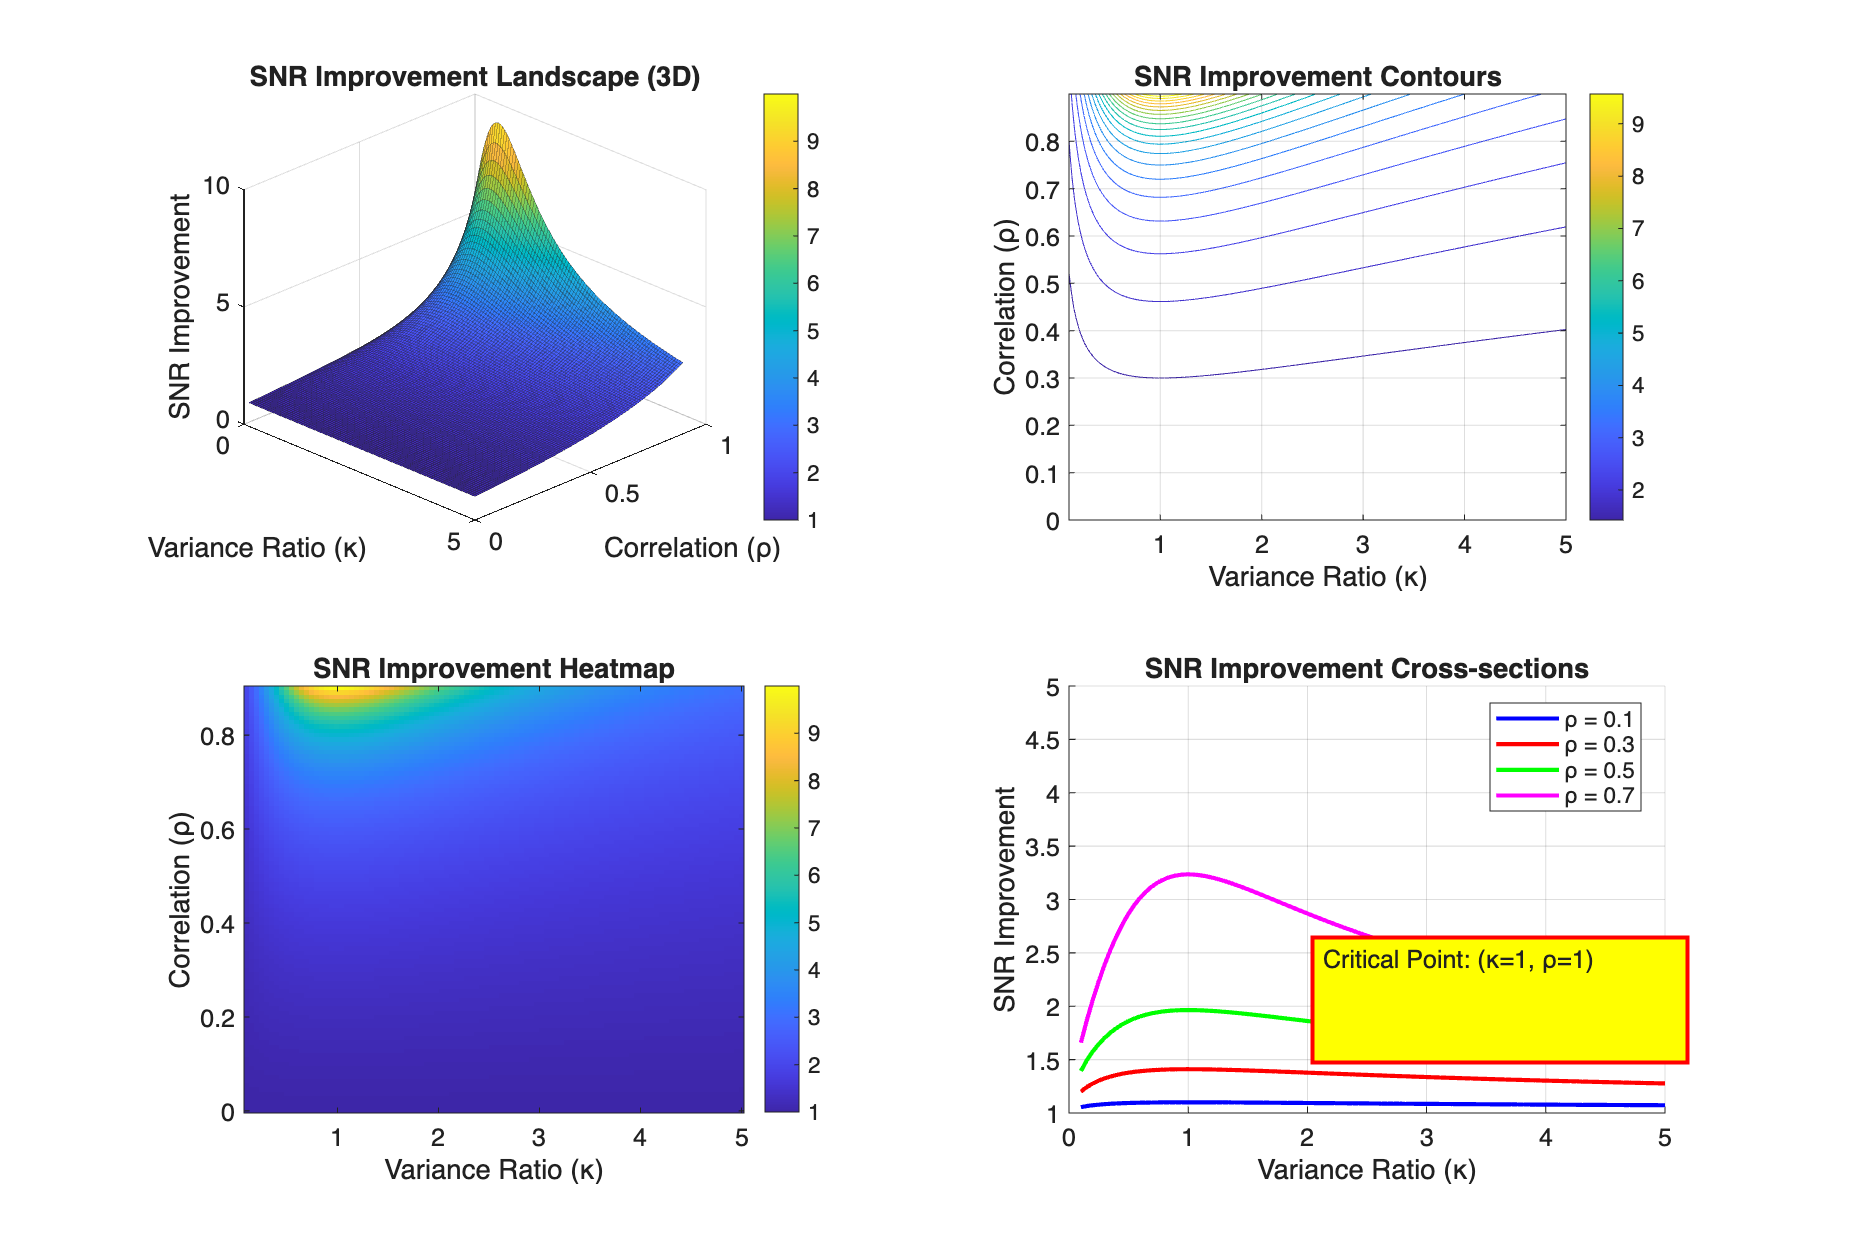
\includegraphics[width=0.9\textwidth]{figures/snr_improvement_landscape.png}
\caption{SNR Improvement Landscape: (a) 3D surface plot, (b) contour plot, (c) heatmap, (d) cross-sections for different correlation values. The landscape shows the relationship between variance ratio $\kappa$, correlation $\rho$, and SNR improvement, with the critical point at ($\kappa=1$, $\rho=1$) highlighted.}
\label{fig:snr_landscape}
\end{figure}

The mathematical foundation draws from information theory \cite{shannon1948mathematical} and statistical estimation theory, providing the theoretical basis for optimal competitive measurement design through correlation exploitation.
